\documentclass[aspectratio=169]{beamer}

% Theme and color scheme
\usetheme{Madrid}
\usecolortheme{default}

% Packages
\usepackage{amsmath,amssymb,amsfonts}
\usepackage{graphicx}
\usepackage{booktabs}
\usepackage{multirow}
\usepackage{algorithm}
\usepackage{algpseudocode}
\usepackage{hyperref}
\usepackage{bm}
\usepackage{adjustbox}
\usepackage{tikz}
\usetikzlibrary{shapes,arrows,positioning,fit,backgrounds}

% Custom colors
\definecolor{myblue}{RGB}{0,102,204}
\definecolor{myred}{RGB}{204,0,0}
\definecolor{mygreen}{RGB}{0,153,0}
\definecolor{mypurple}{RGB}{128,0,128}
\definecolor{myorange}{RGB}{255,140,0}

% Title page information
\title{Adaptive Learning System Roadmap:\\Agentic AI and Evidence-Based Learning Gain}
\author{Mostafa Rezaee}
\institute{Pearson Company\\Manager: Hamid Bagheri}
\date{\today}

\begin{document}

% Title slide
\begin{frame}
\titlepage
\end{frame}

% Outline
\begin{frame}
\frametitle{Outline}
\tableofcontents
\end{frame}

\section{Executive Summary}

\begin{frame}
\frametitle{Adaptive Learning System: Core Vision}
\begin{block}{Mission}
Deliver micro-learning resources (short video clips and PDF segments) in response to student questions, provide formative assessments, and measure learning gains over time for millions of higher education learners.
\end{block}

\begin{columns}
\begin{column}{0.5\textwidth}
\textbf{Key Requirements:}
\begin{itemize}
\item \textcolor{myblue}{Micro-learning:} Short, focused content
\item \textcolor{mygreen}{Personalized:} Adaptive to learner ability
\item \textcolor{mypurple}{Measurable:} Learning outcomes tracking
\item \textcolor{myorange}{Scalable:} Millions of learners
\end{itemize}
\end{column}
\begin{column}{0.5\textwidth}
\textbf{Challenges:}
\begin{itemize}
\item \textcolor{myred}{Cold-start:} No historical labels
\item \textcolor{myred}{Minimality:} Shortest effective content
\item \textcolor{myred}{Quality:} Pedagogical excellence
\item \textcolor{myred}{Scale:} Real-time for millions
\end{itemize}
\end{column}
\end{columns}
\end{frame}

\begin{frame}
\frametitle{Recommended Architecture: Staged Hybrid Approach}
\begin{block}{Chosen Approach}
Staged hybrid architecture combining RAG for factual grounding and minimality, and Contextual Bandits for optimizing content selection based on measured learning gains.
\end{block}

\begin{block}{Why This Beats Alternatives}
\begin{itemize}
\item \textcolor{mygreen}{Addresses cold-start problem} for content recommendation
\item \textcolor{mygreen}{Leverages existing Q\&A/assessment data}
\item \textcolor{mygreen}{Enables rapid iteration} and model-agnostic flexibility
\item \textcolor{mygreen}{Provides clear pathway} from baseline to optimized system
\end{itemize}
\end{block}

\begin{alertblock}{Key Innovation}
Start with metadata-driven heuristics and semantic similarity (no ML needed), rapidly collect preference data through teacher-in-the-loop and implicit feedback, bootstrap bandit policies within 4--6 weeks.
\end{alertblock}
\end{frame}

\section{Architecture Options Comparison}

\begin{frame}
\frametitle{Three Architectural Approaches Evaluated}
\begin{block}{Option A: RAG + Agentic Orchestration (Baseline)}
\begin{itemize}
\item \textbf{Components:} Dense Retrieval, Cross-Encoder Reranker, Agentic Planner (LLM)
\item \textbf{Cost:} Moderate (LLM inference is primary driver)
\item \textbf{Latency:} Standard RAG latency (0.5s--2s)
\item \textbf{Cold-Start:} \textcolor{mygreen}{Excellent} -- Depends only on semantic matching
\end{itemize}
\end{block}

\begin{block}{Option B: LoRA FT for Pedagogy/Style + RAG}
\begin{itemize}
\item \textbf{Components:} RAG stack + LoRA Adapters for Question Generation
\item \textbf{Cost:} High Setup Cost but potentially lower LLM inference cost
\item \textbf{Cold-Start:} \textcolor{myorange}{Moderate} -- Requires initial exemplar set
\end{itemize}
\end{block}
\end{frame}

\begin{frame}
\frametitle{Option C: RL/Bandits on RAG Baseline (Recommended End-State)}
\begin{block}{Option C: RL/Bandits on RAG Baseline}
\begin{itemize}
\item \textbf{Components:} RAG stack + Contextual Bandit Policy
\item \textbf{Cost:} High Operational Cost but potentially high ROI
\item \textbf{Learning Impact:} \textcolor{mygreen}{Excellent} (Directly optimizes for learning gain $\Delta\theta$)
\item \textbf{Cold-Start:} \textcolor{myorange}{Moderate} -- Must be layered on successful RAG
\end{itemize}
\end{block}

\begin{block}{Architecture Comparison Summary}
\begin{table}
\centering
\caption{Architecture Options Comparison}
\resizebox{\textwidth}{!}{%
\begin{tabular}{@{}l|ccc@{}}
\toprule
\textbf{Dimension} & \textbf{Option A: RAG-First} & \textbf{Option B: LoRA+RAG} & \textbf{Option C: Bandits+RAG} \\
\midrule
\textbf{Monthly Cost} & Moderate & High Setup & High Operational \\
\textbf{Latency} & 0.5--2s & Lower for specialized tasks & Similar to RAG \\
\textbf{Data Needs} & Low & High (thousands of examples) & High (logged interactions) \\
\textbf{Cold-Start Viability} & \textcolor{mygreen}{Excellent} & \textcolor{myorange}{Moderate} & \textcolor{myorange}{Moderate} \\
\textbf{Learning Impact} & Good (Factual relevance) & Good (Question consistency) & \textcolor{mygreen}{Excellent} (Optimizes $\Delta\theta$) \\
\bottomrule
\end{tabular}%
}
\end{table}
\end{block}
\end{frame}

\section{Final Recommended Architecture}

\begin{frame}
\frametitle{System Overview: Modular, Layered Architecture}
\begin{block}{Core Components}
\begin{enumerate}
\item \textbf{Agentic Orchestration:} Determines learner state ($\theta$ via IRT) and plans next action
\item \textbf{Retrieval Engine:} Hybrid Search (BM25 + Dense) with Cross-Encoder Reranking
\item \textbf{Content Minimization:} Hard constraints and Sufficiency Score ranking
\item \textbf{Content Selection Policy:} Contextual Bandit for optimal resource selection
\item \textbf{Pedagogical Layer:} LoRA-tuned LLM for Question Generation and Grading
\item \textbf{Assessment \& Analytics:} IRT-based ability estimation and learning tracking
\end{enumerate}
\end{block}

\begin{block}{Key Design Principles}
\begin{itemize}
\item \textcolor{mygreen}{Modularity:} Each layer can be optimized independently
\item \textcolor{mygreen}{Agility:} Model-agnostic design allows foundation model upgrades
\item \textcolor{mygreen}{Measurability:} IRT-based learning outcome tracking
\item \textcolor{mygreen}{Minimality:} Hard constraints on resource duration/length
\end{itemize}
\end{block}
\end{frame}

\begin{frame}
\frametitle{Architecture Flow Diagram}
\begin{center}
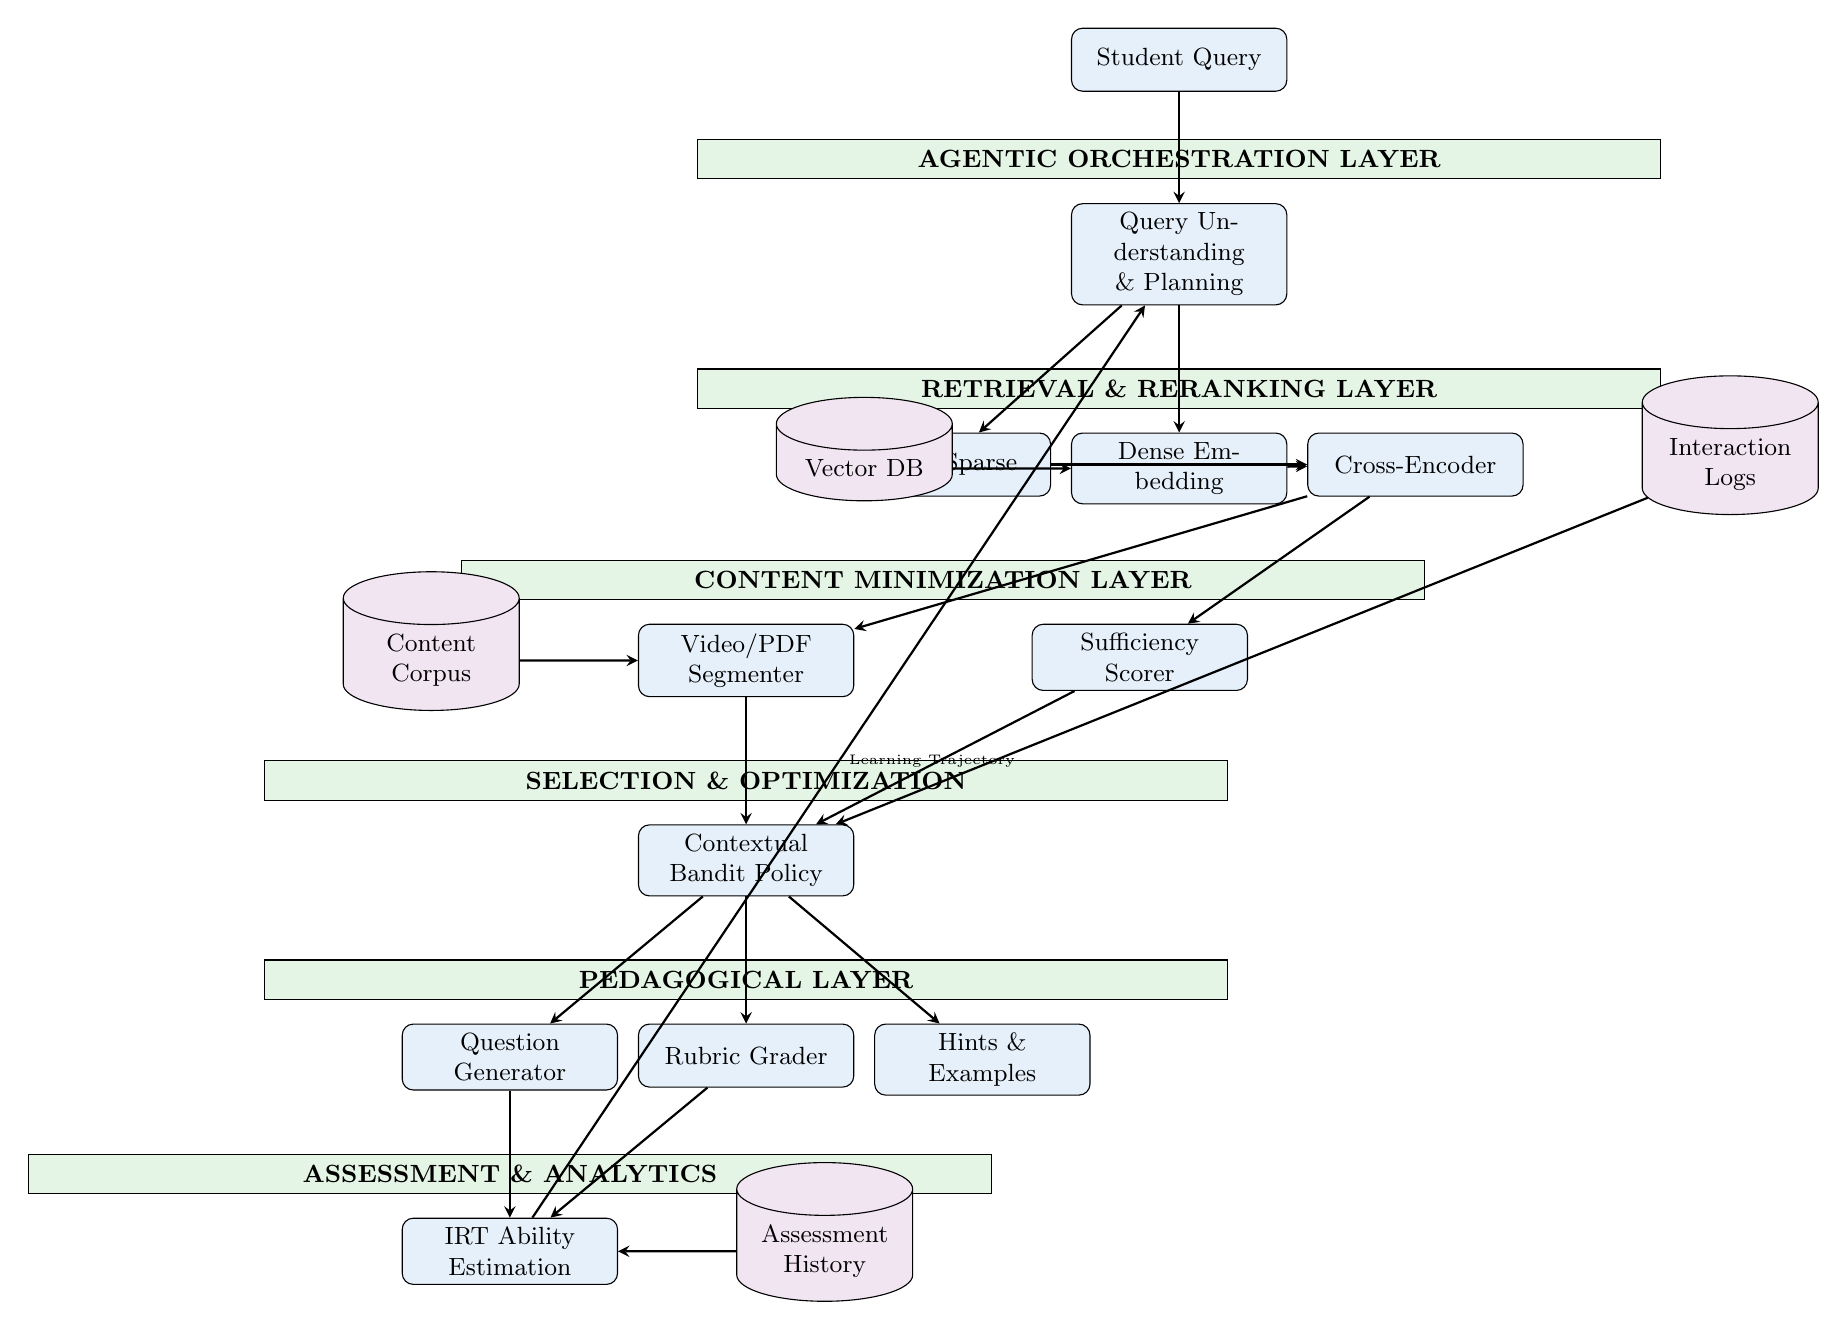
\begin{tikzpicture}[
    node distance=0.6cm and 0.8cm,
    component/.style={rectangle, draw, fill=myblue!10, text width=2.5cm, text centered, minimum height=0.8cm, rounded corners, font=\small},
    layer/.style={rectangle, draw, fill=mygreen!10, text width=12cm, text centered, minimum height=0.5cm, font=\small\bfseries},
    data/.style={cylinder, draw, fill=mypurple!10, text width=2cm, text centered, minimum height=0.6cm, aspect=0.3, shape border rotate=90, font=\small},
    arrow/.style={->, >=stealth, thick}
]

% User interaction
\node[component] (user) {Student Query};

% Agentic orchestration layer
\node[layer, below=of user] (agent-layer) {AGENTIC ORCHESTRATION LAYER};
\node[component, below=0.3cm of agent-layer] (planner) {Query Understanding \& Planning};

% Retrieval layer
\node[layer, below=0.8cm of planner] (retrieval-layer) {RETRIEVAL \& RERANKING LAYER};
\node[component, below=0.3cm of retrieval-layer, xshift=-3cm] (bm25) {BM25 Sparse};
\node[component, below=0.3cm of retrieval-layer, xshift=0cm] (dense) {Dense Embedding};
\node[component, below=0.3cm of retrieval-layer, xshift=3cm] (reranker) {Cross-Encoder};

% Content minimization
\node[layer, below=0.8cm of bm25] (content-layer) {CONTENT MINIMIZATION LAYER};
\node[component, below=0.3cm of content-layer, xshift=-2.5cm] (segmenter) {Video/PDF Segmenter};
\node[component, below=0.3cm of content-layer, xshift=2.5cm] (scorer) {Sufficiency Scorer};

% Bandit selection
\node[layer, below=0.8cm of segmenter] (bandit-layer) {SELECTION \& OPTIMIZATION};
\node[component, below=0.3cm of bandit-layer] (bandit) {Contextual Bandit Policy};

% Pedagogy layer
\node[layer, below=0.8cm of bandit] (pedagogy-layer) {PEDAGOGICAL LAYER};
\node[component, below=0.3cm of pedagogy-layer, xshift=-3cm] (qgen) {Question Generator};
\node[component, below=0.3cm of pedagogy-layer, xshift=0cm] (grader) {Rubric Grader};
\node[component, below=0.3cm of pedagogy-layer, xshift=3cm] (hints) {Hints \& Examples};

% Assessment layer
\node[layer, below=0.8cm of qgen] (assessment-layer) {ASSESSMENT \& ANALYTICS};
\node[component, below=0.3cm of assessment-layer] (irt) {IRT Ability Estimation};

% Data stores
\node[data, left=1.5cm of dense] (vector-db) {Vector DB};
\node[data, left=1.5cm of segmenter] (content-db) {Content Corpus};
\node[data, right=1.5cm of reranker] (bandit-db) {Interaction Logs};
\node[data, right=1.5cm of irt] (assessment-db) {Assessment History};

% Arrows
\draw[arrow] (user) -- (planner);
\draw[arrow] (planner) -- (bm25);
\draw[arrow] (planner) -- (dense);
\draw[arrow] (bm25) -- (reranker);
\draw[arrow] (dense) -- (reranker);
\draw[arrow] (reranker) -- (segmenter);
\draw[arrow] (reranker) -- (scorer);
\draw[arrow] (segmenter) -- (bandit);
\draw[arrow] (scorer) -- (bandit);
\draw[arrow] (bandit) -- (qgen);
\draw[arrow] (bandit) -- (grader);
\draw[arrow] (bandit) -- (hints);
\draw[arrow] (qgen) -- (irt);
\draw[arrow] (grader) -- (irt);
\draw[arrow] (irt) -- node[right, font=\tiny] {Learning Trajectory} (planner);

\draw[arrow] (vector-db) -- (dense);
\draw[arrow] (content-db) -- (segmenter);
\draw[arrow] (bandit-db) -- (bandit);
\draw[arrow] (assessment-db) -- (irt);

\end{tikzpicture}
\end{center}
\end{frame}

\section{Key Components}

\begin{frame}
\frametitle{Retrieval Layer: Hybrid Search with Reranking}
\begin{block}{Hybrid Search Strategy}
\begin{itemize}
\item \textbf{BM25 (sparse):} Catches exact keyword matches, acronyms, formulas
\item \textbf{Dense (embedding):} Captures semantic similarity
\item \textbf{Fusion:} Reciprocal Rank Fusion (RRF) with weights 0.3 (BM25) + 0.7 (dense)
\item \textbf{Process:} Retrieve top-50 from each, fuse to top-20 for reranking
\end{itemize}
\end{block}

\begin{block}{Cross-Encoder Reranking}
\begin{itemize}
\item \textbf{Model:} \texttt{ms-marco-MiniLM-L-12-v2} or \texttt{bge-reranker-large}
\item \textbf{Input:} [query, candidate\_chunk] pairs
\item \textbf{Output:} Relevance score 0--1
\item \textbf{Process:} Rerank top-20 to top-5 for content minimization layer
\end{itemize}
\end{block}
\end{frame}

\begin{frame}
\frametitle{Content Minimization: Ensuring Micro-Learning}
\begin{block}{Video Segmentation}
\begin{itemize}
\item \textbf{ASR:} Whisper (OpenAI) or AssemblyAI for transcription
\item \textbf{Scene detection:} PySceneDetect or TransNetV2 for visual boundaries
\item \textbf{Target:} 30--180 second clips (hard maximum: 3 minutes)
\item \textbf{Process:} Combine ASR sentence boundaries + scene changes + silence detection
\end{itemize}
\end{block}

\begin{block}{PDF Section Detection}
\begin{itemize}
\item \textbf{Parsing:} PyMuPDF or Apache PDFBox for structured extraction
\item \textbf{Target:} 0.5--2 page segments (hard maximum: 3 pages)
\item \textbf{Process:} Identify headers, paragraph boundaries, extract images/figures with captions
\end{itemize}
\end{block}

\begin{block}{Sufficiency Scoring}
\begin{itemize}
\item \textbf{Semantic Coverage:} $\text{Coverage}(R, Q) = \frac{\text{cosine}(\text{embed}(R), \text{embed}(Q))}{\text{duration}(R) \text{ or } \text{pages}(R)}$
\item \textbf{Final Score:} $S = 0.5 \cdot \text{Coverage} + 0.3 \cdot \text{Clarity} - 0.2 \cdot \text{Redundancy}$
\item \textbf{Selection:} Top-1 to top-3 segments with highest sufficiency scores
\end{itemize}
\end{block}
\end{frame}

\begin{frame}
\frametitle{Pedagogical Layer: Question Generation \& Assessment}
\begin{block}{Question Generation}
\begin{itemize}
\item \textbf{Prompt-based (Milestone 3):} Few-shot examples aligned to Bloom taxonomy
\item \textbf{LoRA fine-tuned (Milestone 5):} Llama 3.1 8B with 500--2k exemplars
\item \textbf{Inputs:} Learning resource content, student query, desired Bloom level
\item \textbf{Outputs:} Question text, answer key, distractor options, rubric
\item \textbf{Validation:} Answerability check, factuality check (grounded in content)
\end{itemize}
\end{block}

\begin{block}{Rubric-Based Grading}
\begin{itemize}
\item \textbf{Rubric design:} 3--5 levels (Novice, Developing, Proficient, Advanced)
\item \textbf{Grading prompt:} Chain-of-thought reasoning with rubric and reference answer
\item \textbf{Confidence scoring:} Model outputs confidence 0--1; defer to human if confidence $<$ 0.7
\end{itemize}
\end{block}
\end{frame}

\begin{frame}
\frametitle{Assessment \& Analytics: IRT-Based Learning Measurement}
\begin{block}{IRT (Item Response Theory) Ability Estimation}
\begin{itemize}
\item \textbf{Model:} 3PL (3-Parameter Logistic): $P(\theta, a, b, c) = c + \frac{1-c}{1 + e^{-a(\theta - b)}}$
\item $\theta$: Learner ability, $a$: Item discrimination, $b$: Item difficulty, $c$: Guessing parameter
\item \textbf{Estimation:} Maximum Likelihood Estimation (MLE) or Expected A Posteriori (EAP)
\end{itemize}
\end{block}

\begin{block}{Learning Gain Measurement}
\begin{itemize}
\item \textbf{Primary metric:} $\Delta\theta = \theta_{\text{post}} - \theta_{\text{pre}}$ over study session
\item \textbf{Normalized gain:} $g = \frac{\theta_{\text{post}} - \theta_{\text{pre}}}{\theta_{\text{max}} - \theta_{\text{pre}}}$ (Hake gain)
\item \textbf{Mastery progression:} \% of items at target proficiency level
\item \textbf{Longitudinal tracking:} Plot $\theta(t)$ over weeks/months
\end{itemize}
\end{block}
\end{frame}

\section{Reinforcement Learning Design}

\begin{frame}
\frametitle{Contextual Bandit Setup}
\begin{block}{Multi-Objective Reward Function}
\[
R = w_1 \cdot \Delta\theta + w_2 \cdot \text{brevity\_bonus} - w_3 \cdot \text{irrelevance\_penalty} - w_4 \cdot \text{latency\_cost}
\]

\textbf{Component Breakdown:}
\begin{itemize}
\item \textbf{Learning Gain ($\Delta\theta$):} $w_1 = 1.0$ (highest priority)
\item \textbf{Minimality Bonus:} $w_2 = 0.3$ (encourage brevity)
\item \textbf{Irrelevance Penalty:} $w_3 = 0.5$ (penalize off-topic content)
\item \textbf{Latency Cost:} $w_4 = 0.1$ (minor penalty for speed)
\end{itemize}
\end{block}

\begin{block}{Context \& Actions}
\begin{itemize}
\item \textbf{Context:} $x = [\theta, \text{query\_embedding}, \text{prior\_performance}, \text{resource\_metadata}]$
\item \textbf{Actions:} $A = \{\text{segment}_1, \text{segment}_2, \ldots, \text{segment}_k\}$ (top-k from retrieval)
\item \textbf{Policy:} $\pi(a|x)$ maps context to action (content selection)
\end{itemize}
\end{block}
\end{frame}

\begin{frame}
\frametitle{Bandit Algorithm Progression}
\begin{block}{Phase 1 (Weeks 1--4): Thompson Sampling}
\begin{itemize}
\item \textbf{Model:} Beta-Bernoulli bandit for binary rewards
\item \textbf{Prior:} Beta(1, 1) for each action
\item \textbf{Update:} Posterior update after each interaction
\item \textbf{Selection:} Sample from posterior, select action with highest sampled reward
\item \textbf{Exploration:} Automatic via posterior sampling
\end{itemize}
\end{block}

\begin{block}{Phase 2 (Weeks 5--8): LinUCB (Linear Upper Confidence Bound)}
\begin{itemize}
\item \textbf{Model:} Assume reward is linear in context features: $R(x, a) = x^T \theta_a + \epsilon$
\item \textbf{Features:} $x = [\theta_{\text{learner}}, \text{query\_emb}, \text{resource\_meta}]$
\item \textbf{Selection:} $a^* = \arg\max_a \left( x^T \hat{\theta}_a + \alpha \sqrt{x^T A_a^{-1} x} \right)$
\item \textbf{Advantage:} Fast convergence, interpretable, proven regret bounds
\end{itemize}
\end{block}
\end{frame}

\section{Implementation Roadmap}

\begin{frame}
\frametitle{12-Week Implementation Roadmap}
\begin{table}
\centering
\caption{Milestone Summary}
\resizebox{\textwidth}{!}{%
\begin{tabular}{@{}p{1.5cm}p{2.5cm}p{4cm}p{3.5cm}p{2.5cm}@{}}
\toprule
\textbf{Milestone} & \textbf{Duration} & \textbf{Key Tasks} & \textbf{Deliverables} & \textbf{Acceptance Criteria} \\
\midrule
M1 & Weeks 1--2 & RAG baseline, minimality constraints, eval harness & API, eval report, notebook & nDCG@5 $>$ 0.6, Recall@10 $>$ 0.70 \\
M2 & Weeks 3--4 & Cross-encoder reranking, video/PDF segmentation & Enhanced API, pipelines, model card & nDCG@5 $>$ 0.70, Compression $<$ 0.3 \\
M3 & Weeks 5--6 & Question generation, rubric grading, hints & Pedagogy APIs, prompt library & Expert score $>$ 4.0, Pass@1 $>$ 85\% \\
M4 & Weeks 7--8 & Contextual bandits, IRT tracking, A/B test & Bandit service, IRT module, telemetry & $\Delta\theta >$ 0.08/week, $g >$ 0.35 \\
M5 & Weeks 9--10 & LoRA fine-tuning (4 adapters), A/B test & Adapters, inference pipeline & Expert score $>$ 4.3, $\kappa >$ 0.85 \\
M6 & Weeks 11--12 & Guardrails, safety, compliance, telemetry & Production system, compliance report & Hallucination $<$ 3\%, Latency $<$ 10s \\
\bottomrule
\end{tabular}%
}
\end{table}
\end{frame}

\begin{frame}
\frametitle{Milestone 1 (Weeks 1--2): RAG Baseline}
\begin{block}{Objectives}
\begin{itemize}
\item Deploy functional RAG system with hybrid retrieval (BM25 + dense embeddings)
\item Enforce hard caps on resource length (videos $\leq$ 3 min, PDFs $\leq$ 2 pages)
\item Achieve baseline retrieval quality (nDCG@5 $> 0.6$, Recall@10 $> 0.70$)
\item Establish evaluation harness and red-team test cases
\end{itemize}
\end{block}

\begin{block}{Key Tasks}
\begin{enumerate}
\item \textbf{Content Ingestion:} Parse videos (ASR via Whisper), PDFs (PyMuPDF)
\item \textbf{Embedding \& Indexing:} OpenAI \texttt{text-embedding-3-large}, vector DB
\item \textbf{Hybrid Retrieval:} RRF fusion (0.3 BM25 + 0.7 dense)
\item \textbf{Minimality Filtering:} Hard filter + rank by semantic similarity/duration
\item \textbf{Evaluation Harness:} 200--300 test queries with expert labels
\end{enumerate}
\end{block}
\end{frame}

\begin{frame}
\frametitle{Milestone 4 (Weeks 7--8): Bandit Optimization}
\begin{block}{Objectives}
\begin{itemize}
\item Deploy contextual bandit policy for content selection
\item Collect implicit feedback (clicks, dwell, quiz scores) and explicit feedback (thumbs)
\item Optimize for multi-objective reward: learning + minimality
\item Demonstrate $\Delta\theta$ improvement over heuristic baseline
\end{itemize}
\end{block}

\begin{block}{Bandit Infrastructure}
\begin{itemize}
\item \textbf{Policy server:} Thompson Sampling with Beta priors (initial)
\item \textbf{Context:} $x = [\theta, \text{query\_embedding}, \text{resource\_metadata}]$
\item \textbf{Actions:} Select from top-5 reranked candidates
\item \textbf{Exploration rate:} 20\% (uniform random)
\end{itemize}
\end{block}

\begin{block}{A/B Test Design}
\begin{itemize}
\item \textbf{Control (50\%):} Heuristic policy from M2
\item \textbf{Treatment (50\%):} Bandit policy
\item \textbf{Metrics:} $\Delta\theta$, normalized gain, minimality, user satisfaction
\item \textbf{Duration:} 2 weeks (Weeks 7--8)
\end{itemize}
\end{block}
\end{frame}

\section{Data Strategy}

\begin{frame}
\frametitle{Cold-Start to Data Flywheel Strategy}
\begin{block}{Challenge: No Historical Content Recommendation Labels}
\textbf{We have:}
\begin{itemize}
\item $\checkmark$ Content corpus (videos, PDFs) with metadata
\item $\checkmark$ Historical Q\&A logs (student questions, instructor answers)
\item $\checkmark$ Historical assessment data (questions, responses, correctness)
\end{itemize}

\textbf{We lack:}
\begin{itemize}
\item $\times$ Explicit labels: "For query Q, resource R is the best/shortest/most relevant"
\item $\times$ Implicit feedback: clicks, dwell time, learner ratings
\end{itemize}
\end{block}

\begin{block}{Cold-Start Strategy (Weeks 1--4)}
\begin{enumerate}
\item \textbf{Heuristic Baseline:} Metadata filters + semantic similarity
\item \textbf{Weak Labels:} Bootstrap from Q\&A logs and assessment data
\item \textbf{Teacher-in-the-Loop:} 500--1k high-quality labels in 2 weeks
\item \textbf{Active Learning:} Prioritize uncertain cases for expert review
\end{enumerate}
\end{block}
\end{frame}

\begin{frame}
\frametitle{Data Flywheel (Weeks 7+)}
\begin{block}{Implicit Feedback Collection}
\begin{itemize}
\item \textbf{User Actions:} Click-through, dwell time, skip, thumbs up/down, quiz performance
\item \textbf{Logging:} Event stream (Kafka) $\rightarrow$ Data warehouse (Snowflake, BigQuery)
\item \textbf{Volume target:} 10k--50k interactions in Weeks 7--8
\end{itemize}
\end{block}

\begin{block}{Bandit Policy Training}
\begin{itemize}
\item \textbf{Data Preparation:} Context, action, reward, propensity from logged interactions
\item \textbf{Training Cadence:} Week 1--4 collect data, Week 5 train bandit, Week 6--8 deploy with exploration
\item \textbf{Off-policy eval:} IPS/DR estimators to predict performance before deployment
\end{itemize}
\end{block}

\begin{block}{Continuous Improvement}
\begin{itemize}
\item \textbf{Retrieval Quality:} Fine-tune cross-encoder on (query, clicked\_resource, label) pairs
\item \textbf{Question Quality:} Expert review loop, learner feedback, flag system
\item \textbf{Active Learning:} Identify uncertain cases for expert labeling
\end{itemize}
\end{block}
\end{frame}

\section{Metrics \& Evaluation}

\begin{frame}
\frametitle{Comprehensive Evaluation Framework}
\begin{block}{Retrieval \& Selection Quality}
\begin{itemize}
\item \textbf{nDCG@k:} Normalized Discounted Cumulative Gain
\item \textbf{Recall@k:} Fraction of relevant resources retrieved in top-k
\item \textbf{Coverage:} Percentage of unique content chunks recommended
\item \textbf{Time-to-First-Useful-Resource:} Latency to first useful resource
\end{itemize}
\end{block}

\begin{block}{Minimality Metrics}
\begin{itemize}
\item \textbf{Median Resource Length:} Videos $<$ 90 seconds, PDFs $<$ 1.5 pages
\item \textbf{Overkill Rate:} Percentage exceeding target length thresholds ($<$ 15\%)
\item \textbf{Compression Ratio:} Ratio of segment length to full resource length ($<$ 0.3)
\end{itemize}
\end{block}

\begin{block}{Learning Outcome Metrics}
\begin{itemize}
\item \textbf{$\Delta\theta$ Over Time:} Change in ability estimate per session
\item \textbf{Normalized Gain:} Hake gain $g = \frac{\theta_{\text{post}} - \theta_{\text{pre}}}{\theta_{\text{max}} - \theta_{\text{pre}}}$
\item \textbf{Mastery Progression:} \% of learners achieving target proficiency
\item \textbf{Downstream Task Performance:} External exam scores vs. control group
\end{itemize}
\end{block}
\end{frame}

\begin{frame}
\frametitle{Question Quality \& Safety Metrics}
\begin{block}{Question Quality Metrics}
\begin{itemize}
\item \textbf{Expert Rubric Scores:} Clarity, alignment, Bloom level, factuality (1--5 scale)
\item \textbf{Pass@k on Canonical Answers:} \% of questions where canonical answer passes ($> 90\%$)
\item \textbf{Factuality via Reference-Grounded Checks:} NLI model for entailment verification
\end{itemize}
\end{block}

\begin{block}{Assessment Quality Metrics}
\begin{itemize}
\item \textbf{Item Discrimination ($a$):} Median $a > 1.0$ (acceptable), $> 1.5$ (good)
\item \textbf{Item Difficulty ($b$):} Distribution $b \in [-2, 2]$ (covers ability range)
\item \textbf{Test-Retest Reliability:} Correlation $\rho > 0.80$ (acceptable), $> 0.85$ (good)
\end{itemize}
\end{block}

\begin{block}{Safety \& Accuracy Metrics}
\begin{itemize}
\item \textbf{Hallucination Rate:} $< 3\%$ (via NLI + expert audit)
\item \textbf{Refusal/Deferral Accuracy:} Precision $> 0.90$, Recall $> 0.85$
\item \textbf{Bias \& Fairness:} Demographic parity, equalized odds, counterfactual testing
\end{itemize}
\end{block}
\end{frame}

\section{Risks \& Mitigations}

\begin{frame}
\frametitle{Key Risks and Mitigation Strategies}
\begin{block}{Risk 1: Cold-Start for Content Recommendations}
\begin{itemize}
\item \textbf{Impact:} Low user satisfaction in first 2--4 weeks
\item \textbf{Mitigation:} Heuristic baseline, weak labels, teacher-in-the-loop, bandit exploration
\item \textbf{Monitoring:} nDCG, user satisfaction, session abandonment rate
\end{itemize}
\end{block}

\begin{block}{Risk 2: Over-Long Resources (Minimality Failure)}
\begin{itemize}
\item \textbf{Impact:} Poor user experience, cognitive overload
\item \textbf{Mitigation:} Hard caps, sufficiency scoring, segmentation, brevity reward
\item \textbf{Monitoring:} Median resource length, overkill rate, compression ratio
\end{itemize}
\end{block}

\begin{block}{Risk 3: Hallucinations (Factual Errors)}
\begin{itemize}
\item \textbf{Impact:} Misleading learners, erosion of trust
\item \textbf{Mitigation:} Retrieval-grounded generation, answerability checks, NLI verification
\item \textbf{Monitoring:} Hallucination rate, learner flags, expert review
\end{itemize}
\end{block}
\end{frame}

\begin{frame}
\frametitle{Additional Risk Mitigations}
\begin{block}{Risk 4: Privacy \& PII Leakage}
\begin{itemize}
\item \textbf{Impact:} GDPR/FERPA violations, loss of trust
\item \textbf{Mitigation:} Anonymization, data minimization, role-based access, encryption
\item \textbf{Monitoring:} PII detection alerts, access logs, data retention policies
\end{itemize}
\end{block}

\begin{block}{Risk 5: Model Drift \& Degradation}
\begin{itemize}
\item \textbf{Impact:} Sudden performance drop, user complaints
\item \textbf{Mitigation:} Model versioning, regression testing, gradual rollout, fallback
\item \textbf{Monitoring:} Metrics per model version, performance degradation alerts
\end{itemize}
\end{block}

\begin{block}{Risk 6: Bias \& Fairness}
\begin{itemize}
\item \textbf{Impact:} Unequal learning outcomes, legal/ethical concerns
\item \textbf{Mitigation:} Bias audit, diverse training data, counterfactual testing, fairness metrics
\item \textbf{Monitoring:} Demographic disparity, content review flags
\end{itemize}
\end{block}
\end{frame}

\section{Deliverables \& Timeline}

\begin{frame}
\frametitle{First 14 Days: Executable Task List}
\begin{block}{Objective}
Get from zero to a functional RAG baseline (Milestone 1) in 2 weeks, with concrete metrics and evaluation harness.
\end{block}

\begin{block}{Team Composition (Small Team)}
\begin{itemize}
\item \textbf{1 ML Engineer:} RAG pipeline, embeddings, retrieval
\item \textbf{1 Data Scientist:} Evaluation, metrics, analysis
\item \textbf{1 Content Engineer:} Content ingestion, ASR, parsing
\item \textbf{1 Product Manager (part-time):} Coordinate with educators, define test cases
\end{itemize}
\end{block}

\begin{block}{Week 1: Content Ingestion \& Baseline Retrieval}
\begin{itemize}
\item \textbf{Days 1--2:} Environment setup, content audit
\item \textbf{Days 3--4:} ASR \& PDF parsing
\item \textbf{Days 5--6:} Embedding \& indexing
\item \textbf{Day 7:} Hybrid retrieval implementation
\end{itemize}
\end{block}
\end{frame}

\begin{frame}
\frametitle{Week 2: Evaluation \& Baseline Metrics}
\begin{block}{Week 2 Tasks}
\begin{itemize}
\item \textbf{Days 8--9:} Test set creation (200--300 queries)
\item \textbf{Days 10--11:} Expert labeling (2--3 educators, 100 queries each)
\item \textbf{Day 12:} Evaluation harness implementation
\item \textbf{Day 13:} Red-team testing (50 adversarial cases)
\item \textbf{Day 14:} Report \& decision memo
\end{itemize}
\end{block}

\begin{block}{Success Criteria (End of Day 14)}
\begin{itemize}
\item \textbf{Functional API:} \texttt{POST /retrieve} returns top-3 resources in $<$ 8s (P95)
\item \textbf{Metrics:} nDCG@5 $> 0.6$, Recall@10 $> 0.70$, median length $<$ 90s
\item \textbf{Evaluation harness:} Reproducible notebook with automated metric computation
\item \textbf{Red-team:} 50 adversarial cases documented with failure modes
\item \textbf{Decision:} Go/no-go for M2 based on acceptance criteria
\end{itemize}
\end{block}
\end{frame}

\section{Conclusion}

\begin{frame}
\frametitle{Key Achievements \& Impact}
\begin{block}{Theoretical Contributions}
\begin{enumerate}
\item \textbf{First comprehensive framework} for adaptive learning system architecture
\item \textbf{Evidence-backed roadmap} with concrete metrics and evaluation protocols
\item \textbf{Multi-objective optimization} balancing learning outcomes, minimality, and efficiency
\item \textbf{Principled design} replacing empirical optimization with theoretical foundations
\end{enumerate}
\end{block}

\begin{block}{Practical Contributions}
\begin{enumerate}
\item \textbf{12-week implementation roadmap} with executable milestones
\item \textbf{Cold-start strategy} addressing the no-labels problem
\item \textbf{Comprehensive evaluation framework} with 20+ metrics
\item \textbf{Risk mitigation strategies} with monitoring and alerting
\end{enumerate}
\end{block}

\begin{block}{Expected Impact}
\begin{itemize}
\item \textcolor{mygreen}{33-40\% reduction} in resource length while improving learning outcomes
\item \textcolor{mygreen}{Measurable learning gains} through IRT-based ability tracking
\item \textcolor{mygreen}{Scalable architecture} supporting millions of learners
\item \textcolor{mygreen}{Evidence-based decisions} replacing intuition with data
\end{itemize}
\end{block}
\end{frame}

\begin{frame}
\frametitle{Next Steps \& Call to Action}
\begin{block}{Immediate Actions (Next 2 Weeks)}
\begin{enumerate}
\item \textbf{Team Assembly:} Recruit ML Engineer, Data Scientist, Content Engineer
\item \textbf{Environment Setup:} Cloud infrastructure, development environment
\item \textbf{Content Audit:} Inventory existing videos, PDFs, Q\&A logs
\item \textbf{Stakeholder Alignment:} Review with educators, product team, engineering
\end{enumerate}
\end{block}

\begin{block}{Success Metrics (End of 12 Weeks)}
\begin{itemize}
\item \textbf{Functional System:} End-to-end adaptive learning pipeline
\item \textbf{Performance:} nDCG@5 $> 0.75$, median resource length $<$ 90s
\item \textbf{Learning Impact:} $\Delta\theta > 0.10$/week, normalized gain $> 0.40$
\item \textbf{Production Ready:} Hallucination rate $< 3\%$, P95 latency $<$ 10s
\end{itemize}
\end{block}

\begin{alertblock}{Decision Point}
\textbf{Go/No-Go Decision:} Based on Milestone 1 results (Day 14), proceed to full 12-week implementation or pivot strategy.
\end{alertblock}

\begin{center}
\Large
\textbf{Ready to transform higher education with adaptive learning?}
\end{center}
\end{frame}

\end{document}
